\section{Method: The GAST Forecaster}
\label{sec:method}

\subsection{Overview and design principles}

GAST (Gap-Aware Spatio-Temporal forecaster) is a masked-history encoder coupled to a goal-conditioned multimodal decoder. Its organisation follows from a single decision: the validity mask is not an input channel that accompanies the coordinates, but the generator of an explicit \emph{observation-evidence state} that every subsequent stage reads. Three principles follow.

\textbf{P1: Evidence is hierarchical, not local.} Whether a frame is trustworthy depends on how long ago the agent was last seen. The evidence state is therefore a function of the missing run age, and it is shared by all stages instead of being recomputed independently by each module.

\textbf{P2: Unobserved agents may listen but must not speak.} A currently unobserved pedestrian can still be predicted from its neighbours, but its stale position must not be offered to other agents as current evidence. This asymmetry is enforced in the relational attention.

\textbf{P3: The decoder starts where the evidence ends.} The forecast origin may be several frames after the last observation. The decoder is anchored at the last observed position and is told the elapsed gap, so that its first predicted point is consistent with the (unknown) unobserved interval rather than being tied to a placeholder row.

Figure~\ref{fig:arch} summarises the resulting architecture. The encoder consists of a frame-wise relational stage (GERE) and an evidence-conditioned causal temporal stage (ECTA); the decoder predicts, for each of $K=20$ modes, an endpoint relative to the anchor and a residual trajectory conditioned on that endpoint. No stage receives an imputed coordinate.

\begin{figure*}[t]
\centering
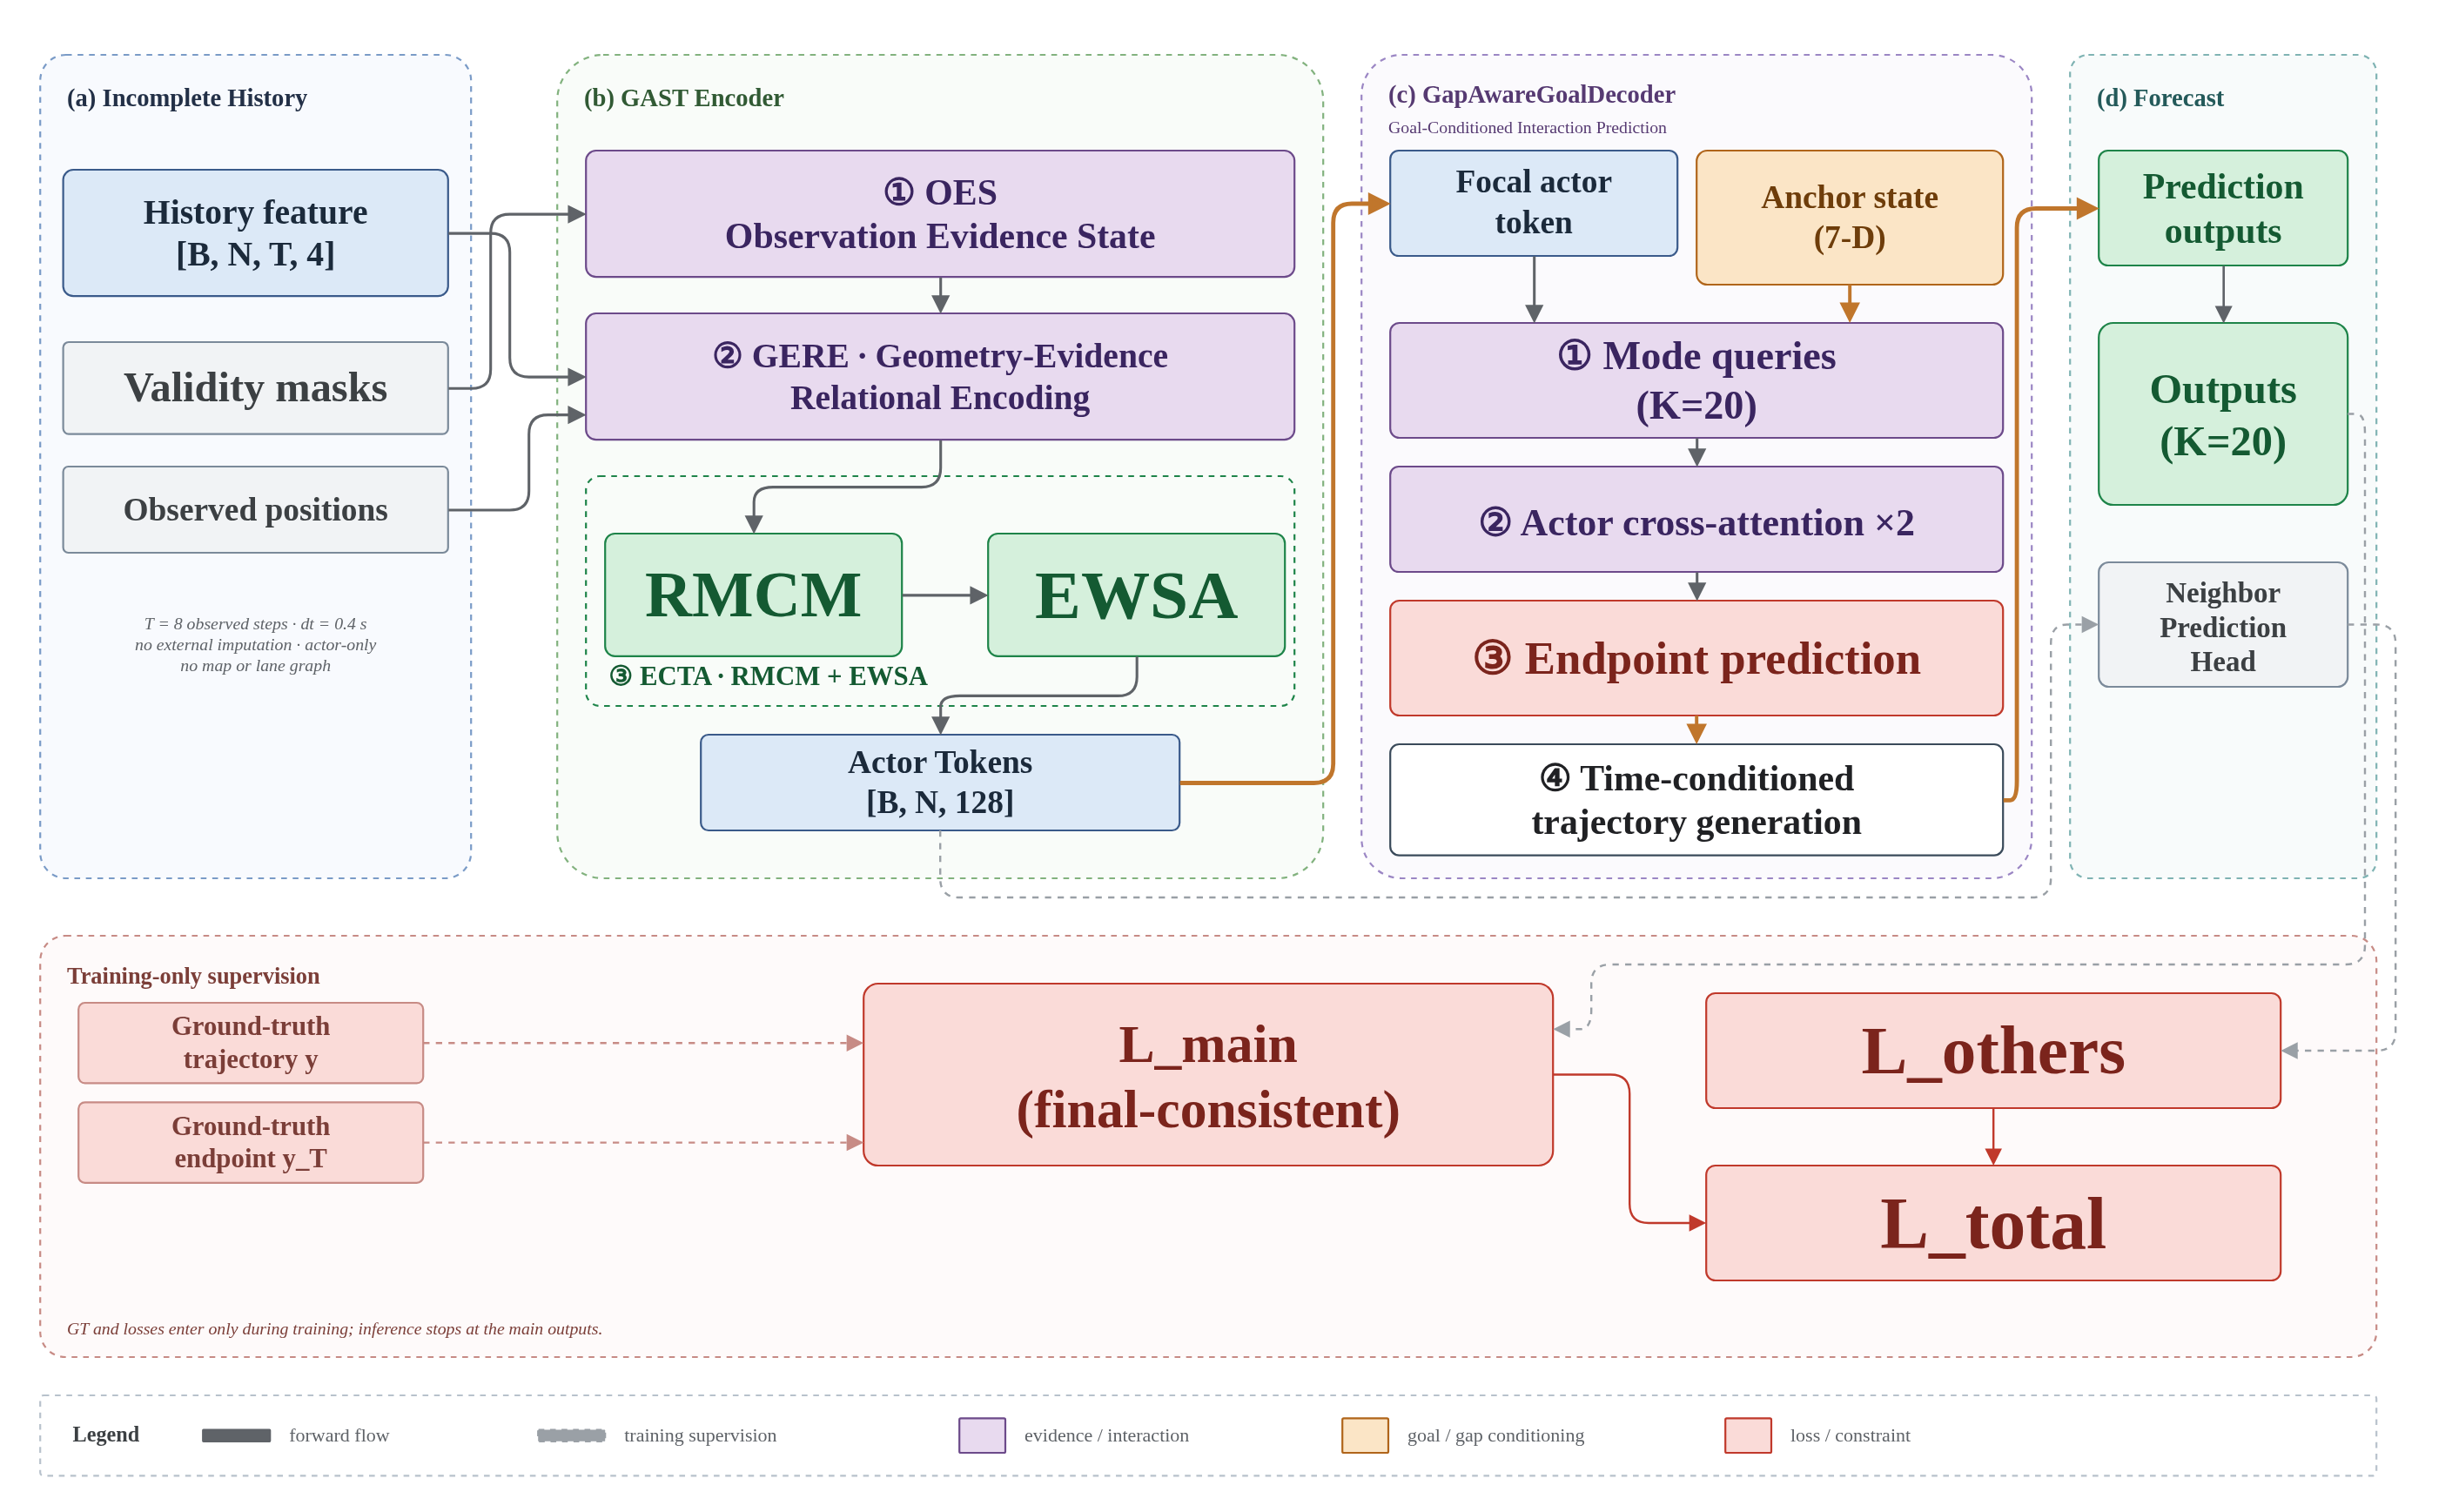
\includegraphics[width=0.94\textwidth]{figures/architecture_crop.png}
\caption{Architecture of GAST. (a)~The masked history is represented by positions, validity masks and observed positions only; missing entries are placeholders. (b)~The observation-evidence state (OES) drives GERE, which performs frame-wise relational attention with geometry bias and source eligibility, and ECTA, which scales the temporal input by evidence strength (RMCM) and aggregates states with an evidence-weighted readout (EWSA). (c)~The goal-conditioned decoder builds a seven-dimensional anchor state from the last observed frame, forms $K$ mode queries and predicts an endpoint plus a progress-conditioned residual per mode. (d)~Outputs are $K$ trajectories with probabilities and per-mode scales; the neighbour head is used only during training.}
\label{fig:arch}
\end{figure*}

\subsection{Observation-evidence state}
\label{sec:oes}

For pedestrian $i$ at history step $t$, let
\begin{equation}
a_{i,t}=t-\max\{t'\le t: m_{i,t'}=1\},
\label{eq:age}
\end{equation}
be the age of the most recent observation, with $a_{i,t}=t$ when no frame up to $t$ has been observed (a virtual observation is assumed immediately before the window). The state comprises three quantities: the eligibility $s_{i,t}=m_{i,t}$ that decides whether the frame may act as a source of evidence, the age $a_{i,t}$, and a reliability
\begin{equation}
r_{i,t}=m_{i,t}+(1-m_{i,t})\,\exp(-\tau\,a_{i,t}),\qquad \tau=\mathrm{softplus}(\vartheta),
\label{eq:reliability}
\end{equation}
with a single learnable scalar $\vartheta$ initialised so that $\tau\approx0.1$. Reliability is exactly one at observed frames and decays monotonically over a gap. Padded agents are excluded from the state, and $r$ is zero for them.

Two properties of \eqref{eq:reliability} matter. First, it is not a calibrated probability and we never interpret it as one: it is a task-internal reliability variable whose role is to order history states by evidential support. Second, it is an identity on fully observed histories ($r\equiv1$), so the evidence conditioning vanishes and GAST reduces to its backbone. This is what allows the model to be compared with complete-history architectures without a distribution shift.

\subsection{GERE: frame-wise relational encoding with geometry bias}
\label{sec:gere}

The per-frame input of agent $i$ is a four-dimensional vector
\begin{equation}
u_{i,t}=\big[\Delta p_{i,t},\ \Delta s_{i,t},\ m_{i,t}\big],
\label{eq:input}
\end{equation}
containing the position increment, the increment of the observed speed, and the validity flag, mapped by a patch embedding $h_{i,t}=\mathrm{PatchEmbed}(u_{i,t})$.

\textbf{Ghost token.} At each frame the model pools the validity pattern of the whole scene into a single token,
\begin{equation}
g_{t}=\mathrm{max}_{i\in\mathcal{V}_{t}}\ \psi\big(\mathbf{1}-m_{i,t}\big),
\label{eq:ghost}
\end{equation}
where $\psi$ is a two-layer embedding applied to the scalar mask broadcast over the channel dimension and $\mathcal{V}_{t}$ is the set of non-padded agents. The token is prepended to the $N$ agent tokens for that frame and removed after attention. Because its input is the mask and only the mask, it summarises \emph{who is currently observable} without carrying any positional content; it therefore cannot inject a phantom coordinate, but it does give every agent a shared description of the scene's current observability.

\textbf{Source eligibility.} Attention keys are restricted to the ghost token and to agents with $s_{j,t}=1$. All agents, including unobserved ones, remain valid queries. An unobserved agent can therefore read the current state of its neighbours and the scene summary, but its own stale feature is never attended to by others. This implements P2 and differs from simply adding the mask as a feature, which leaves a stale token in the key set.

\textbf{Geometry bias.} For every ordered pair $(i,j)$ the model computes a seven-dimensional relational descriptor from the observed geometry,
\begin{equation}
f_{ij,t}=\big[\Delta p_{ij},\ \log(1+\|\Delta p_{ij}\|),\ \Delta v_{ij},\ \cos\Delta\theta_{ij},\ \sin\Delta\theta_{ij}\big],
\label{eq:geom}
\end{equation}
where $\Delta p_{ij}=p_{j,t}-p_{i,t}$, $\Delta v_{ij}=v_{j,t}-v_{i,t}$ and $\Delta\theta_{ij}$ is the difference of heading angles. Velocities are estimated from the current observation and the previous \emph{observed} position, divided by the number of steps between them, so a gap does not create a spurious velocity spike; if either endpoint of the pair is unobserved, $f_{ij,t}=\mathbf{0}$. The descriptor is mapped to one bias per attention head,
\begin{equation}
B_{ij,t}^{(h)}=w_{2}^{(h)\top}\,\mathrm{GELU}\big(W_{1}f_{ij,t}\big),
\label{eq:bias}
\end{equation}
and added to the attention logits of the agent--agent block. The output projection of \eqref{eq:bias} is zero-initialised, so training starts from a geometry-agnostic relational encoder and the bias is learned only if it reduces the objective. The relational stage is applied per frame; its output is a sequence of spatial states for each agent.

\subsection{ECTA: evidence-conditioned causal temporal aggregation}
\label{sec:ecta}

\textbf{RMCM (reliability-modulated causal encoder).} The spatial states are projected and scaled by the reliability before entering a causal recurrence,
\begin{equation}
\tilde{x}_{i,t}=\mathrm{MLP}(x_{i,t})\cdot r_{i,t},
\qquad
u_{i,1:T}=\mathrm{SSM}_{\phi}(\tilde{x}_{i,1:T}),
\label{eq:rmcm}
\end{equation}
where $\mathrm{SSM}_{\phi}$ is a stack of four unidirectional selective state-space blocks \cite{gu2023mamba}. Causality is required because the forecast must not depend on future history positions, and it makes the encoder usable in streaming deployment. The modulation is a scalar per frame and channel-shared: it changes how strongly a state enters the recursion, not what the state represents. In particular, an observed frame enters with unit strength, whereas a frame that has been missing for three steps is attenuated by $e^{-3\tau}$ and is effectively prevented from overwriting the last reliable state with a decayed one.

\textbf{EWSA (evidence-weighted state aggregation).} Readout is not fixed to the last time step. With content scores $e_{i,t}=w^{\top}u_{i,t}$ and a temperature $\beta=1$, the model forms
\begin{equation}
\alpha_{i,t}=\mathrm{softmax}_{t}\big(e_{i,t}+\beta\log r_{i,t}\big),\qquad
\bar{h}_{i}=\sum_{t}\alpha_{i,t}\,u_{i,t},
\label{eq:ewsa}
\end{equation}
and gates the terminal state against this aggregate,
\begin{equation}
z_{i}=r_{i,T}\,u_{i,T}+\big(1-r_{i,T}\big)\bar{h}_{i}.
\label{eq:gate}
\end{equation}
When the last frame is observed, $z_{i}=u_{i,T}$ exactly and the readout is identical to a standard terminal readout. When it is missing, the model falls back to a weighted average of the available states, with the weights shaped both by learned content and by evidence strength. The gate is a hard switch in form but a soft one in value, since $r_{i,T}$ decays continuously with the terminal gap.

\subsection{Anchor-conditioned goal decoding}
\label{sec:decoder}

\textbf{Anchor state.} Let $\ell_{i}$ be the index of the last observed frame and $\ell'_{i}$ the index of the previous one. The decoder receives
\begin{equation}
\varphi_{i}=\Big[p_{i,\ell_i},\ v_{i},\ \tfrac{\delta_{i}}{T},\ \rho_{i},\ \mathbb{1}[\ell_{i}<T]\Big]\in\mathbb{R}^{7},
\label{eq:anchor}
\end{equation}
where $\delta_{i}=T-\ell_{i}+1$ is the number of steps from the last observation to the forecast origin, $v_{i}=(p_{i,\ell_i}-p_{i,\ell'_i})/(\ell_i-\ell'_i)$ is a gap-aware velocity (zero when only one frame is observed), $\rho_{i}=\frac{1}{T}\sum_{t}m_{i,t}$ is the observed fraction, and the last term marks terminal missingness. The anchor position is retained so that the module is defined in any coordinate frame; under the anchor-centred normalisation of Section~\ref{sec:task} it vanishes and the state is carried by the velocity and gap descriptors.

\textbf{Mode queries.} The pedestrian representation $z_{i}$ from \eqref{eq:gate} and the anchor embedding $e^{\varphi}_{i}=\mathrm{MLP}(\varphi_{i})$ are combined with a learned per-mode embedding $e_{k}$,
\begin{equation}
q_{i,k}=z_{i}+e^{\varphi}_{i}+e_{k},\qquad k=1,\dots,K,
\label{eq:query}
\end{equation}
and refined by two cross-attention layers over the scene's pedestrian tokens, with padded agents masked out. Each mode thus sees the context under its own anchor condition rather than sharing a single scene vector.

\textbf{Endpoint and trajectory.} A head maps each mode query to a displacement from the anchor,
\begin{equation}
\hat{y}_{i,k,H}=p_{i,\ell_i}+\Delta_{i,k},\qquad \Delta_{i,k}=\mathrm{MLP}(q_{i,k}).
\label{eq:endpoint}
\end{equation}
For step $t=1,\dots,H$, let $\tau_{t}=\delta_{i}+t-1$ be the elapsed steps between the anchor time and that future step, and let $p_{t}=\tau_{t}/(\delta_{i}+H-1)$ be the corresponding fraction of the anchor-to-endpoint interval. The trajectory is a straight skeleton plus a decaying residual,
\begin{equation}
\hat{y}_{i,k,t}=p_{i,\ell_i}+p_{t}\,\Delta_{i,k}+\big(1-p_{t}\big)\,g_{\psi}\big(q_{i,k},e(\Delta_{i,k}),e(\tau_{t}\Delta t)\big).
\label{eq:traj}
\end{equation}
The construction has three consequences. The first predicted point is already advanced along the skeleton by $\delta_{i}/(\delta_{i}+H-1)$, so a long terminal gap is not silently treated as if the pedestrian had waited at the last observed position. The residual has full freedom early in the horizon and vanishes exactly at $t=H$, so the endpoint of the output coincides with the predicted goal. And because $p_{t}$ is defined in units of the actual gap, the same module handles observed and terminal-missing samples without a special case.

\textbf{Mode probabilities and scales.} A scoring head reads the mode query, the endpoint embedding and the mean of the per-step queries, and produces logits whose softmax gives $\pi_{i,k}$. A parallel head outputs a per-step, per-axis Laplace scale $\sigma_{i,k,t}=\mathrm{ELU}(\cdot)+1.0001$, used by the likelihood term below; $\sigma$ is a dispersion parameter of the predicted distribution, not a calibrated confidence interval.

\subsection{Training objective}
\label{sec:loss}

Supervision is applied to the focal pedestrian (index 0 of each scene sample). For mode $k$ we compute the average displacement $d_{k}$ and the endpoint error $d^{\mathrm{end}}_{k}$ against the ground truth, and define the joint error $J_{k}=d_{k}+\lambda_{e}d^{\mathrm{end}}_{k}$ with $\lambda_{e}=1$. Two different modes are selected for two different purposes: the regression mode $k^{\ast}=\arg\min_{k}J_{k}$ balances shape and destination, while the classification target $k^{\dagger}=\arg\min_{k}d_{k}$ is defined by trajectory-level error alone. The loss is
\begin{equation}
\mathcal{L}=\mathcal{L}_{\mathrm{reg}}+\mathcal{L}_{\mathrm{cls}}
+\mathcal{L}_{\mathrm{NLL}}+\mathcal{L}_{\mathrm{end}}
+\lambda_{d}\mathcal{L}_{\mathrm{div}}+\mathcal{L}_{\mathrm{nbr}},
\label{eq:loss}
\end{equation}
where $\mathcal{L}_{\mathrm{reg}}=\mathrm{SmoothL1}(\hat{y}_{k^{\ast}},y)$, $\mathcal{L}_{\mathrm{cls}}=-\log\pi_{k^{\dagger}}$, $\mathcal{L}_{\mathrm{end}}=\mathrm{SmoothL1}(\hat{y}_{k^{\ast},H},y_{H})$, $\mathcal{L}_{\mathrm{nbr}}=\mathrm{SmoothL1}(\hat{y}^{\mathrm{nbr}},y^{\mathrm{nbr}})$, and $\mathcal{L}_{\mathrm{div}}=\mathbb{E}_{k\ne l}[0.5-\|\hat{y}_{k,H}-\hat{y}_{l,H}\|]_{+}$ is a hinge on pairwise endpoint distances; $\mathcal{L}_{\mathrm{NLL}}$ is the Laplace negative log-likelihood detailed in Appendix~\ref{app:loss}. The cross-entropy is evaluated with label smoothing $0.2$, the diversity weight is $\lambda_{d}=0.05$, and the margin is $0.5$~m. The likelihood term is computed on the trajectory-closest mode, $\log(2\sigma)+|y-\hat{y}|/\sigma$ averaged over steps and axes, combined with a soft-target cross-entropy $0.5\sum_{k}\tilde{\pi}_{k}\log\pi_{k}$ whose target $\tilde{\pi}$ is a temperature-softmax of the negative trajectory errors; it calibrates the dispersion and gently shapes the mode distribution without competing with the hard classification target. The neighbour term predicts the future of the other agents in the scene from their encoder states and is used only during training; at inference the model returns the $K$ candidate futures of the focal pedestrian and their probabilities.

The separation of $k^{\ast}$ and $k^{\dagger}$ is deliberate. Probability should rank modes by how well they explain the whole trajectory, whereas the endpoint head should be trained on the mode that best explains the destination. Sharing a single assignment forces one objective to compromise; separating them costs nothing at inference.

\subsection{Properties}

\textbf{Exact reduction.} With $m_{i,t}=1$ for all $t$, \eqref{eq:reliability} gives $r\equiv1$: \eqref{eq:rmcm} becomes a plain causal encoder, \eqref{eq:gate} returns the terminal state, and the anchor state carries only the observed velocity, with $\delta=1$, $\rho=1$ and no terminal flag. The gap-specific machinery therefore contributes nothing in this condition, and any difference from a complete-history baseline is attributable to the decoder and to the always-present scene-level token.

\textbf{No leakage.} Placeholders never enter a difference, a distance or a velocity: velocities are computed only between observed frames, pairwise geometry is zeroed when either endpoint is unobserved, and unobserved agents are removed from the key set. Ground-truth futures are used only in the loss.

\textbf{Cost.} The model has 1.19M parameters (0.60M encoder, 0.55M decoder), and inference is a single forward pass with $K=20$ parallel mode queries; no sampling loop is required. Per-frame relational attention is $O(N^{2})$ in the number of pedestrians in a frame, which is the same order as the social-attention baselines we compare against.
